%%
%% This is file `./samples/longsample.tex',
%% generated with the docstrip utility.
%%
%% The original source files were:
%%
%% apa7.dtx  (with options: `longsample')
%% ----------------------------------------------------------------------
%% 
%% apa7 - A LaTeX class for formatting documents in compliance with the
%% American Psychological Association's Publication Manual, 7th edition
%% 
%% Copyright (C) 2021 by Daniel A. Weiss <daniel.weiss.led at gmail.com>
%% 
%% This work may be distributed and/or modified under the
%% conditions of the LaTeX Project Public License (LPPL), either
%% version 1.3c of this license or (at your option) any later
%% version.  The latest version of this license is in the file:
%% 
%% http://www.latex-project.org/lppl.txt
%% 
%% Users may freely modify these files without permission, as long as the
%% copyright line and this statement are maintained intact.
%% 
%% This work is not endorsed by, affiliated with, or probably even known
%% by, the American Psychological Association.
%% 
%% ----------------------------------------------------------------------
%% 
\documentclass[man]{apa7}

\usepackage{lipsum}

\usepackage[american]{babel}

\usepackage{caption} % For captioning outside figures
\usepackage{capt-of} % For captioning outside figures

\usepackage{siunitx}
\usepackage{matlab-prettifier}

\usepackage{csquotes}
\usepackage[style=apa,backend=biber]{biblatex}
\addbibresource{bibliography.bib}

\title{Parking Occupancy Detection from CCTV Images}
\shorttitle{}
\authorsnames{Jule Valendo Halim -1425567}
\authorsaffiliations{GEOM90038 - Advanced Imaging}

\begin{document}

\maketitle
\tableofcontents
\newpage
\section{Introduction}

Recent developments in data has undergone significant changes from data processing into machine learning due to increased volumes of readily available data (\textcite{KHAN20201444}). The introduction of image-based neural network architecture has allowed the field of computer vision to flourish. Computer vision leverages the power of machine learning to derive meaningful information from visual data, which allows them to take actions and recommendations when they detect issues. Powerful advances in machine learning such as the widely popular transformer model that Chat-GPT is based on has also been adapted to be trained on visual information (\textcite{elnouby2021training}). Figure \ref{fig:representationNeuralNetwork} provides a representation of a neural network, which consists of multiple layers. The input layer is the initial data, and hidden layers calculate the weights of each of these data and propagates them forward to other hidden layers. Finally, the output layer provides probabilities of the desired output (e.g., some classification label).

\begin{minipage}{\linewidth}
  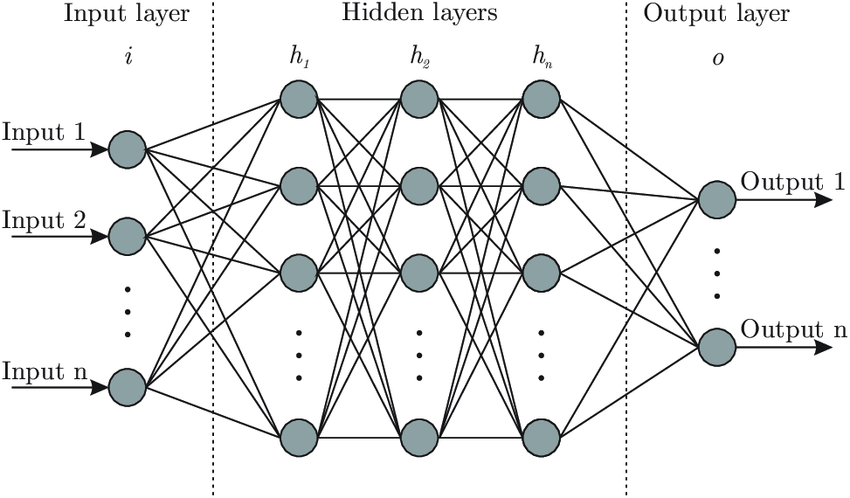
\includegraphics[height=\textheight/4 ,width=\textwidth/1]{figures/sampleNeuralNetwork.png}
  \captionof{figure}{Visual Representation of Layers That Makes Up a Neural Network (\textcite{neuralNetwork})}
  \label{fig:representationNeuralNetwork}
\end{minipage}

Figure \ref{fig:exampleArchitecture} provides a simplified neural network architecture for visual data. The visual data that is placed into the input layer depends on the specific architecture and design. In the case of figure \ref{fig:exampleArchitecture}, a section of the image is placed into the input layer. It is then propagated forward towards additional layers before finally obtaining the results of the output layer, which in this case, attempts to classify the image into four possible species.

\begin{minipage}{\linewidth}
  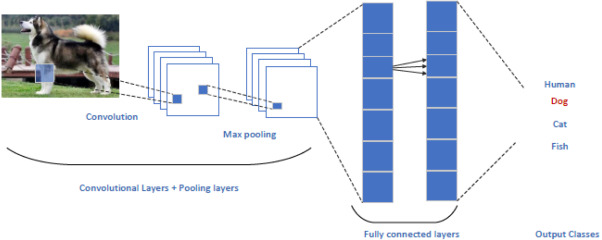
\includegraphics[height=\textheight/4 ,width=\textwidth/1]{figures/exampleML.jpg}
  \captionof{figure}{Sample Architecture of Machine Learning Being Used in Computer Vision (\textcite{CHAI2021100134})}
  \label{fig:exampleArchitecture}
\end{minipage}

The use of computer vision has been applied to wide range of different fields. For example, \textcite{MEDICAL} discussed the way medical imaging applications in multiple medical areas such as pathology and dermatology has enhanced the level of care provided. Another field in which machine learning has enhanced computer vision is in the automation and digitization of fruit quality measuring and maintainence (\textcite{SUPERMARKET}). Figure \ref{fig:exampleDetection} shows how computer vision can be used to detect cars and humans in images. These detections are generated post-training, where multiple images are provided for training the neural network. The trained neural network can then be given new images or even real time video to detect what they were trained to. However, as seen in figure \ref{fig:exampleDetection}, such neural networks are not perfect, and can misclassify or not detect parts of the image that they are supposed to (e.g., the model did not successfully classify one of the humans walking).

\newpage

\begin{minipage}{\linewidth}
  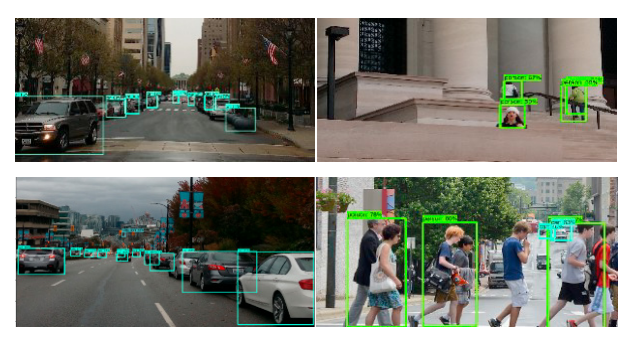
\includegraphics[height=\textheight/4 ,width=\textwidth/2]{figures/detectionExample.png}
  \captionof{figure}{Sample Image Detection Results of Cars and People Using Deep Learning and RCNN Models(\textcite{KHAN20201444})}
  \label{fig:exampleDetection}
\end{minipage}

Faster Recurrent Neural Network models (FasterRCNN model) are a form of neural network that can detect objects in images. The FasterRCNN model is based off \textcite{fasterRCNN}. It consists of two main components, the Region Proposal Network (RPN) and the FastRCNN. RPNs are a convolutional neural network, which are a form of neural network such as those described above, but are specialized in taking three dimensional data (such as images) as inputs. RPNs are further specialized to handle different schemas of different images. Figure \ref{fig:RPN} shows the different schemas that the RPN can handle, namely differing scales, differing filter sizes, and multiple references of the same image. 

\begin{minipage}{\linewidth}
  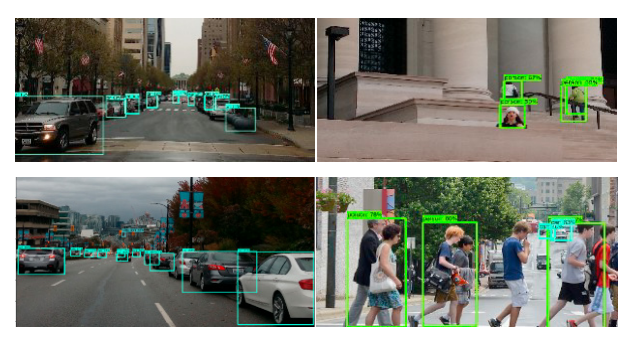
\includegraphics[height=\textheight/4 ,width=\textwidth/2]{figures/detectionExample.png}
  \captionof{figure}{Different Schemas that RPNs Are Adapted To(\textcite{fasterRCNN})}
  \label{fig:RPN}
\end{minipage}

\newpage

The other component, the FastRCNN (\textcite{fastRCNN}) is a neural network that has been shown to be much faster than other image detection neural networks. The main innovation that causes this increased detection speed is the use of of Regions of Interest (RoI). The RoI is defined with a four-tuple (r,c,h,w). The r and c specifies the top-left corner, while the h and w defines its height and width respectively. These tuples are then max-pooled to convert features inside regions of interest into a small feature map with fixed spatial size (e.g., height and width of 6 x 7). Figure \ref{fig:ROI} shows the overall architecture of the fastRCNN. As seen in this figure, the image is projected into an RoI format before being pooled and trained on a neural network.

\begin{minipage}{\linewidth}
  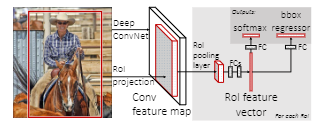
\includegraphics[]{figures/ROI.png}
  \captionof{figure}{The FastRCNN Architecture, Including the Conversion of Images into ROI(\textcite{fastRCNN})}
  \label{fig:ROI}
\end{minipage}

The FasterRCNN architecture has layers that provide output towards the RPN. This is then used to create a proposal, which basically proposes what sort of schema the image is using (see figure \ref{fig:RPN}). The image that is passed through the RPN is also used to create feature maps, which create is then passed to the the RoI pooling before being passed to a classifier. In this architecture, the RPN is performing the 'attention' task of FasterRCNN. Attention allows the model to incorporate sequential information into the model (e.g., in a picture of a man on a horse, the model is able to remember that the section of the image with a hat is in the upper-middle area of the whole image). Figure \ref{fig:fasterRCNNArchitecture} shows the entirety of the FasterRCNN architecture.

\newpage

\begin{minipage}{\linewidth}
  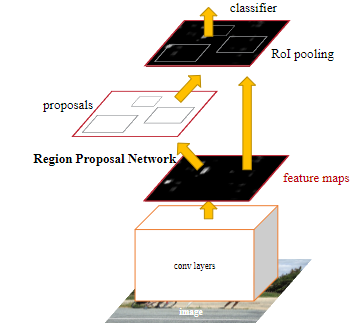
\includegraphics[height=\textheight/4 ,width=\textwidth/2]{figures/fasterRCNN2.png}
  \captionof{figure}{The FasterRCNN Architecture, Showing the Components of RPN and FastRCNN RoI (\textcite{fasterRCNN})}
  \label{fig:fasterRCNNArchitecture}
\end{minipage}

The other model used in this report is the Resnet50 CNN model (\textcite{resnet50}). The Resnet50 CNN model's building block consists of a series of weight layers that have an relu activation function (an activation function converts the weights provided by the layer mapped to an output). Relu takes the maximum of two values and returns an output depending on the input (e.g., a relu that is max(0,x) and has a binary classification task to classify 0 and 1 would classify an output as 1 if x is greater than 0, and classify it as 0 if it is less than 0). Figure \ref{fig:resnet50} shows the building block layer of the Resnet50. The Resnet50 CNN consists of multiple of these layers along with other kinds of layers, one of which is the max-pool layer. This increased depth of representation is vital for visual recognition tasks, and this model is popular in many visual recognition tasks.

\begin{minipage}{\linewidth}
  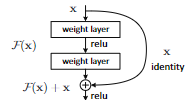
\includegraphics[height=\textheight/6 ,width=\textwidth/4]{figures/resnet.png}
  \captionof{figure}{The Resnet50 CNN Building Block (Layer)(\textcite{resnet50})}
  \label{fig:resnet50}
\end{minipage}

\newpage

In this report, I aim to use and investigate a pre-trained FasterRCNN model and Resnet50 CNN model(trained on the PKPlot dataset) to detect cars and delineate parking spaces in a picture of the Barry Street parking lot. The software used will be MATLAB 2020a, along with additional toolboxes such as the deep learning toolbox. The methodology of this begins with a visualization of the dataset, before using a pre-trained Resnet50 CNN classifier to create a classifier. Afterwards, parking slot delineation is done using FasterRCNN. The dataset for this step involves images of the parking slot and bounding boxes, which identifies the space in which an object is identified (see figure \ref{fig:exampleDetection}, where cars and human areas and identified using bounding boxes).

These results will then be evaluated by calculating recall and precision. These metrics are calculated as 

\[
\text{Precision} = \frac{TP}{TP + FP} \quad \text{where } TP = \text{True Positives, } FP = \text{False Positives}
\]
\[
\text{Recall} = \frac{TP}{TP + FN} \quad \text{where } TP = \text{True Positives, } FN = \text{False Negatives}
\]

Afterwards, the object performance will be post-processed to improve the resulting classification. Visual inspection of the resulting bounding boxes will also be compared to the ground truth of where bounding boxes should be. Additional information is found in the methods and results section. The entirety of the code is found in appendix D. However, relevant parts of the code will be written throughout the report.

\newpage

\section{Methods and Results}

\subsection{Visualizing Dataset}
This step involves loading in the PKPlot and Barry Street annotated images. These annotations are bounding boxes that are manually set. Figure \ref{fig:datasetImages} shows the annotated images of the PKPlot (left) and Barry Street (right) datasets. The PKPlot dataset consists of over 695,000+ parking space images. For this report, only a segment of the total dataset was used.

\begin{minipage}{\linewidth}
  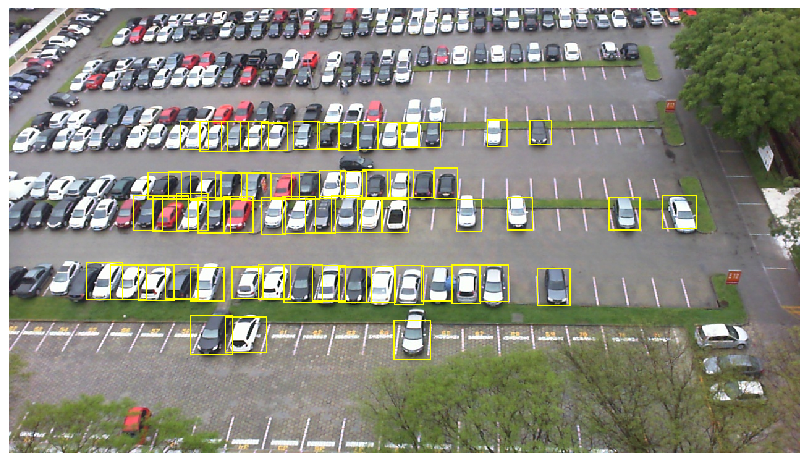
\includegraphics[height=\textheight/4,width=\textwidth/2]{figures/pkplot.png}
  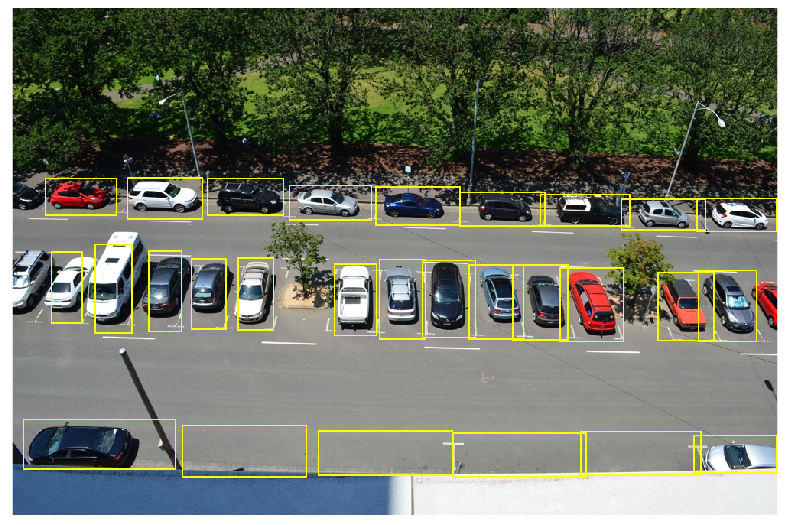
\includegraphics[height=\textheight/4,width=\textwidth/2]{figures/barrystreet.png}
  \captionof{figure}{Images of Annotated from the PKPlot Dataset (left) and Barry Street Dataset (right)}
  \label{fig:datasetImages}
\end{minipage}

Figure \ref{fig:pkplot2} shows a sample empty slot and occupied slot found in the annotated PKPlot datasets.

\begin{minipage}{\linewidth}
  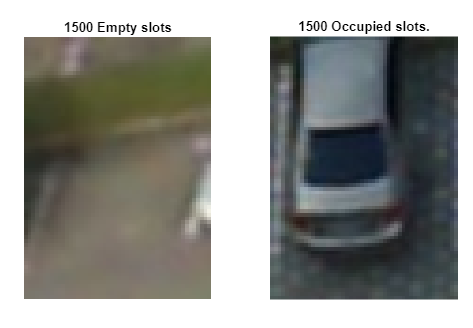
\includegraphics[height=\textheight/4,width=\textwidth/2]{figures/pkplot2.png}
  \captionof{figure}{Sample Image of Empty (left) and Occupied (right) Slots of PKPlot, Sampled From 1500 Empty Spaces and 1500 Occupied Spaces}
  \label{fig:pkplot2}
\end{minipage}


\subsection{Creating Car Detector}

\subsubsection{Re-Training the Resnet50 CNN Model on PKPlot Dataset}
To create the car detector, the pre-trained Resnet50 CNN was used. The model was set to train on 70\% of the dataset, and 30\% was kept as the validation set. The classication layer of the model with a different classification layer that predicts two classes, occupied and empty parking spaces. An additional augmented dataset was also created, which involves two changes, rotating and changing the scales of the original image. This would allow the model to be trained on a larger dataset as well as being able to generalize to unseen car images (e.g., if the same car was rotated, the model can still identify it). The model was then re-trained with the new models. Figure \ref{fig:modelTraining} shows the loss and accuracy of the model over 20 epochs. The loss and accuracy converge at around 5-8 epochs, with the model obtaining near perfect accuracy and nearly no loss on both the validation and test data.

\begin{minipage}{\linewidth}
  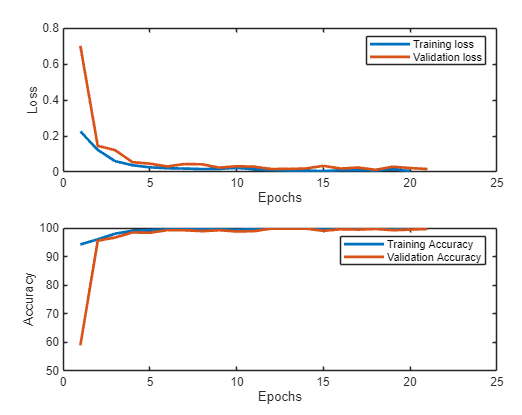
\includegraphics[height=\textheight/4,width=\textwidth/2]{figures/carDetector.png}
  \captionof{figure}{Loss (up) and Accuracy (down) on Validation and Training Datasets, Re-Trained Model on PKPlot}
  \label{fig:modelTraining}
\end{minipage}

\subsubsection{Testing the Model on Barry Street Dataset}
The same model was then used to identify the same labels (occupied and empty parking spaces) on the Barry Street dataset. Figure \ref{fig:confMatrix} shows the confusion matrix of the re-trained model on the Barry Street dataset. It was able to correctly identify the empty and occupied spaces with high accuracy, correctly identifying 99.2\% of the parking spaces (20.4\% were correctly identified as empty and 78.8\% were correctly identified as occupied). 0.8\% of the predictions were incorrect. The model appears to be able to predict occupied areas more accurately than empty areas (100\% accuracy in classifying occupied targets and 96.5\% accuracy is classifying empty spaces).

\begin{minipage}{\linewidth}
  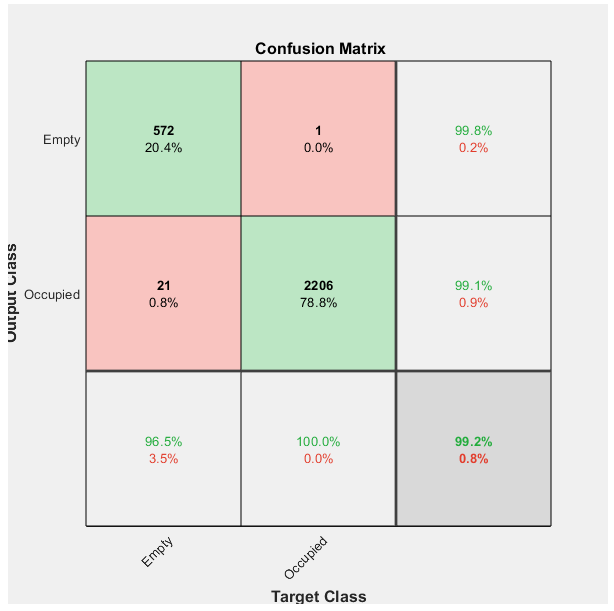
\includegraphics[height=\textheight/4,width=\textwidth/2]{figures/confMatrix.png}
  \captionof{figure}{Confusion Matrix of Re-Trained Resnet50 CNN Model on Barry Street Data}
  \label{fig:confMatrix}
\end{minipage}

Figure \ref{fig:wrongPred} shows the visualizations of the 21 incorrectly predicted areas, along with their target scores. A target score of greater than 0.5 for each label indicates that it classifies that space as that label (e.g., an occupied score of 0.6763 means that the model predicted that the model is 67.63\% confident that the area is occupied, and the reverse is also true for empty scores). As seen from the figure, occupied scores are generally much higher, meaning that the model was very confident in their wrong predictions of an area being occupied, compared to empty scores, which only has a empty score of 0.58, which does not show high confidence in that prediction.

\newpage

\begin{minipage}{\linewidth}
  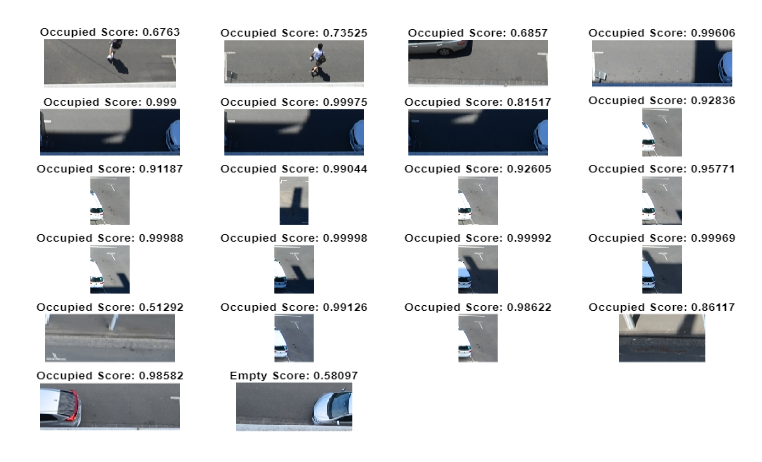
\includegraphics[height=\textheight/2,width=\textwidth/1]{figures/wrongPred.png}
  \captionof{figure}{Visualization of 21 (0.8\% of the total dataset) wrong predictions, along with their target scores}
  \label{fig:wrongPred}
\end{minipage}

\subsection{Automatic Delineation of Parking Spaces}

\subsubsection{Re-Training the FasterRCNN on PKPlot}

This section uses the FasterRCNN pre-trained model that was trained on detection of cars in highways from a mounted camera on a car. It has been shown to be able to predict cars in highways well, but on still CCTV images, the performance is questionable. Similar to the re-training done on the Restnet50 CNN, the FasterRCNN is re-trained on the PKPlot dataset to identify cars and parking spaces. The initial model's performance is shown in figure \ref{fig:modelIterations}. The graphs plot the model performance over iterations. The first graph (from top left) shows the training loss, which is close to 0. The second and third graphs show the results of the RPN layer, both accuracy and RMSE. The last two graphs show the overall model's accuracy and RMSE.

\begin{minipage}{\linewidth}
  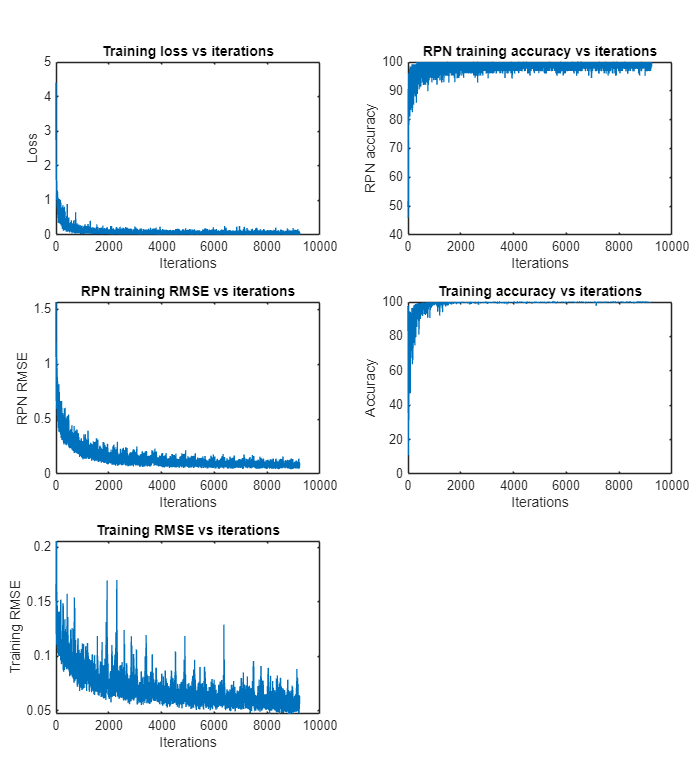
\includegraphics[height=\textheight/2,width=\textwidth/1]{figures/modelIteration.png}
  \captionof{figure}{Results of Re-Training FasterRCNN on PKPlot}
  \label{fig:modelIterations}
\end{minipage}

\subsubsection{Visualizing Re-Trained Model Predictions}

To visualize the prediction results of the model, the predicted areas in which the model classifies as having a car is shown in figure \ref{fig:bStreetPredictions}. The yellow bounding boxes have the confidence scores as well (similar to the scores in \ref{fig:wrongPred}) The prediction confidence are generally quite high, with most correctly identified parking spaces having a confidence of above 0.9, with one exception of the car at the bottom right. However, this car is also cut off and so could contribute to the reduced confidence. Nevertheless, the model was not able to identify all the cars, even in areas where the cars are fully in frame. The car was also unable to correctly identify any empty parking spaces in the image. 

\begin{minipage}{\linewidth}
  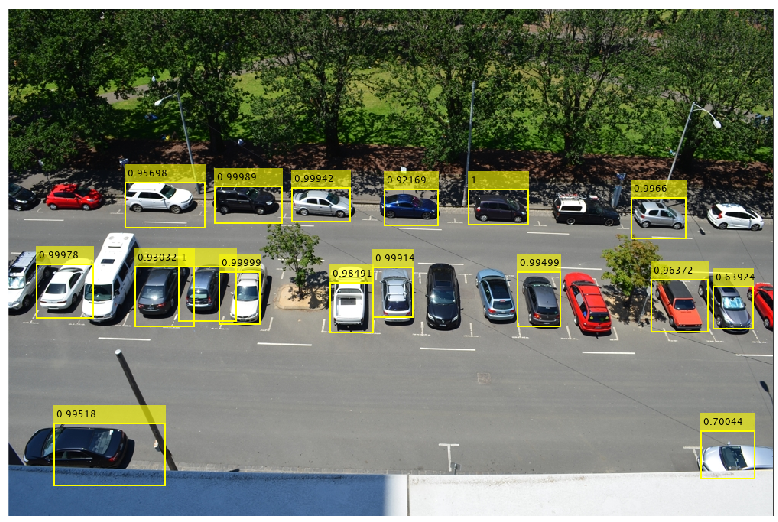
\includegraphics[height=\textheight/2,width=\textwidth/1]{figures/modelPredictions.png}
  \captionof{figure}{FasterRCNN Predictions on the Barry Street}
  \label{fig:bStreetPredictions}
\end{minipage}

\subsubsection{Improving Model Prediction}

To improve the model to correctly identify more cars, the model was further trained on more frames from the Barry Street CCTV. The predicted bounding boxes on all the frames were clustered and drawn. Figure \ref{fig:clusterBox} shows the clusters represented as scatter points and bounding boxes.

\newpage

\begin{minipage}{\linewidth}
  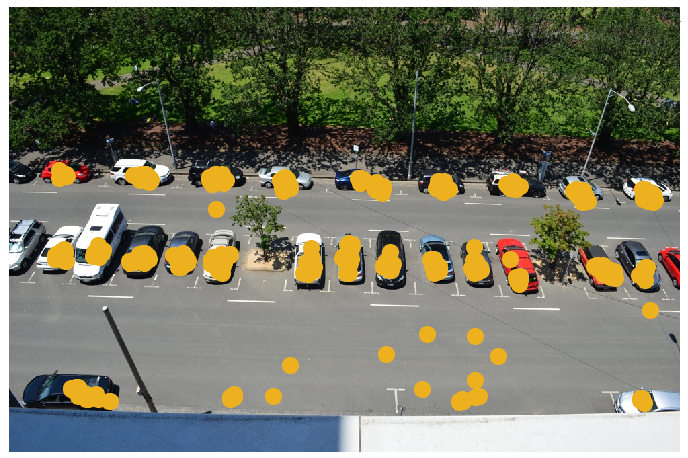
\includegraphics[height=\textheight/4,width=\textwidth/2]{figures/clusterDot.png}
  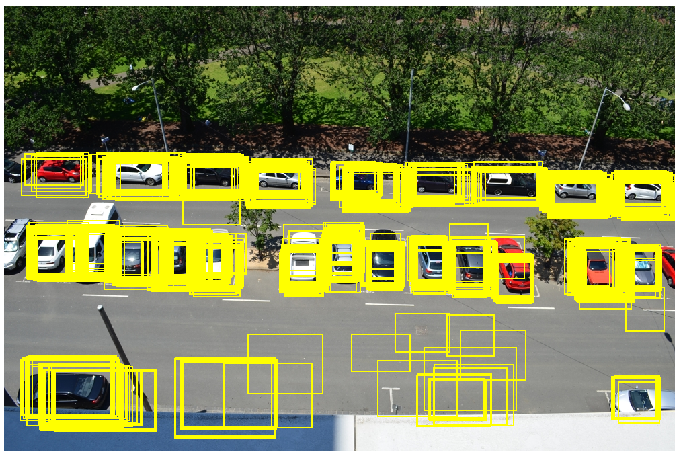
\includegraphics[height=\textheight/4,width=\textwidth/2]{figures/clusterBox.png}
  \captionof{figure}{Predicted bounding box clusters of all frames, shown as scatter points (left) and boxes (right)}
  \label{fig:clusterBox}
\end{minipage}

The bounding boxes (figure \ref{fig:clusterBox} (right)) then had their classification scores averaged and plotted. Figure \ref{fig:clusterAvg} shows the resulting averaged cluster and the corresponding classification scores.

\begin{minipage}{\linewidth}
  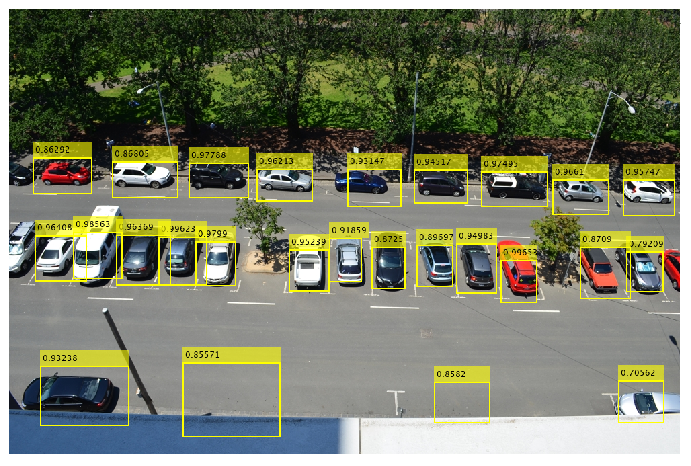
\includegraphics[height=\textheight/2,width=\textwidth/1]{figures/clusterAvg.png}
  \captionof{figure}{Averaged Bounding Boxes and the Corresponding Classification Scores}
  \label{fig:clusterAvg}
\end{minipage}

\subsection{Evaluation}

\subsubsection{Evaluation Steps and Code}

To perform evaluation on the resulting averaged predictions, the recall and precisions are calculated. The predicted data is structured as a dataset where each row consists of [x coordinates, y coordinates, length, width] of the bounding box. A ground truth dataset that contains the same structure as the predictions were given, and is used for the evaluation calculations described above. The evaluation steps and corresponding code are:

1. Displaying the means of the bounding boxes described in figure \ref{fig:clusterAvg}.

\begin{lstlisting}[]
% x(1), y(2), length(3), width(4)
disp(classifiedMean)
\end{lstlisting}

The resulting table displayed is shown in appendix A, along with additional mean calculations for the width and length. \newline

2. Adjusting the x and y positions of the bounding boxes in (1) by a shift of 141 pixels along the x axis and 58 pixels on the y axis.

\begin{lstlisting}[]

adjustedClassifiedMean=classifiedMean
adjustedClassifiedMean(:,1)=adjustedClassifiedMean(:,1)-141
adjustedClassifiedMean(:,2)=adjustedClassifiedMean(:,2)-58

\end{lstlisting}

The resulting table of adjusted bounding box X and Y coordinates are shown in appendix B. \newline

\newpage

3. Create and input the table in a format for the 'evaluateDetectionPrecision' function.

\begin{lstlisting}[]

detectionResults = table('Size',[1,2], ...
'VariableTypes',{'cell','cell'}, ...
'VariableNames', {'Boxes','Scores'})
detectionResults.Boxes{1} = adjustedClassifiedMean;
detectionResults.Scores{1} = classifiedScoreMean;
disp(detectionResults)

\end{lstlisting}


4. Load the ground truth data and create a table similar to step (3)

\begin{lstlisting}[]

load("FinalCode\GroundTruthBarryStreet.mat")
groundTruthData = table('Size',[1,1], ...
'VariableTypes',{'cell'}, ...
'VariableNames', {'Boxes'})
groundTruthData.Boxes{1} = ParkingSlots

\end{lstlisting}

5. Obtain the precision and recall of adjusted bounding boxes and plot the results.

\begin{lstlisting}[]

[averagePrecision, recall, precision] = 
    evaluateDetectionPrecision(detectionResults, groundTruthData)
figure;
plot(recall, precision,'-x');
xlabel('Recall');
ylabel('Precision');
title(['Average Precision = ' num2str(averagePrecision) ]);
grid on;

\end{lstlisting}

\subsubsection{Evaluation Results}

Table \ref{fig:adjustedPrecRec1} shows the resulting precision and recall calculations on the adjusted X and Y positions. 

\begin{minipage}{\linewidth}
  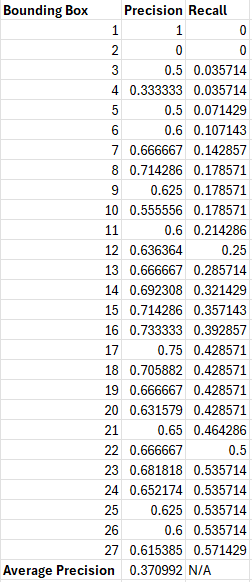
\includegraphics[]{figures/avgPrecRec.png}
  \captionof{figure}{Table of Precision, Average Precision, and Recall of Adjusted Bounding Box Predictions}
  \label{fig:adjustedPrecRec1}
\end{minipage}

Figure \ref{fig:adjustedPrecRec2} shows the resulting plot of precision and recall. The average precision is 0.37099.

\newpage

\begin{minipage}{\linewidth}
  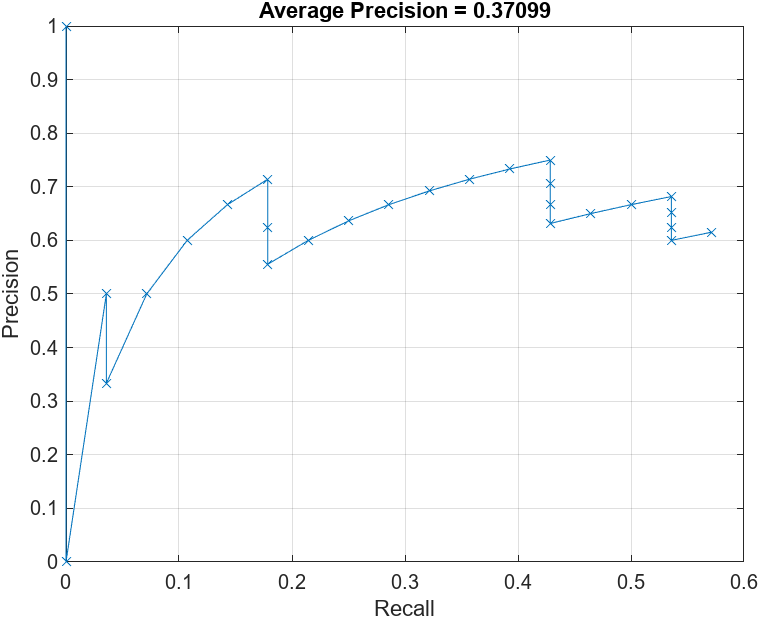
\includegraphics[height=\textheight/2,width=\textwidth/1]{figures/graph.png}
  \captionof{figure}{Plotted Recall vs Precision}
  \label{fig:adjustedPrecRec2}
\end{minipage}

To obtain a visualization of the errors in the predictions, the ground truth bounding boxes are plotted agains the adjusted predictions.

\begin{lstlisting}[]
figure;
xlim([0, 1100]);
ylim([0, 650]);
set(gca, 'YDir', 'reverse')
hold on;

for i = 1:size(adjustedClassifiedMean,1)
    rectangle('Position', adjustedClassifiedMean(i,:), 'EdgeColor',
     'black', 'LineWidth', 1);
end

for i = 1:size(ParkingSlots,1)
    rectangle('Position', ParkingSlots(i,:), 'EdgeColor', 'r', 
    'LineWidth', 1);
end
hold off;
\end{lstlisting}

Figure \ref{fig:unimprovedBoxes} shows the plotted bounding boxes of the predicted bounding boxes (black) and the ground truth boxes (red). As this figure shows, the predicted areas are very different from the ground truth boxes. To improve this, post-processing improvements will be done in the next section to improve the precision and recall of the predictions by adjusting the predicted bounding boxes to more accurately match the ground truth.

\newpage

\begin{minipage}{\linewidth}
  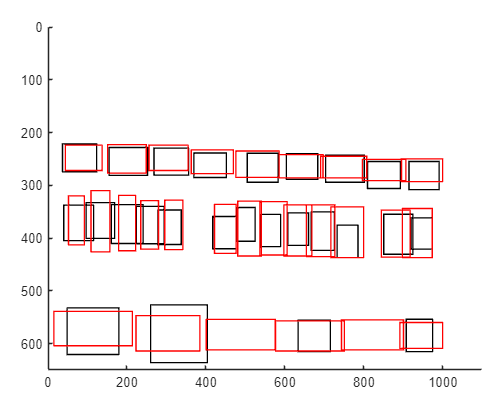
\includegraphics[]{figures/plottedBoxesUnimproved.png}
  \captionof{figure}{Plotted Bounding Boxes of Unimproved Predictions (black) Plotted Against Ground Truth Bounding Boxes (red)}
  \label{fig:unimprovedBoxes}
\end{minipage}

\subsection{Post-Processing Improvements}

\subsubsection{Plotting Bounding Box Sizes}

To visualize the different bounding box sizes, the predicted bounding boxes are plotted. To ensure that the orientation of each bounding boxes are the same, the aspect ratios of each box was calculated. If it was greater than 1, the x and y coordinates are swapped, along with their widths and lengths. This effectively orients each box to be 'vertically' oriented (the length is shorter than the width for each box). The code to plot the boxes and the swaps are shown below. 

\newpage

\begin{lstlisting}[]

figure;
hold on;
axis equal;
xlim([0, 200]);
ylim([0, 200]);
xlabel('Width of parking slots in pixels');
ylabel('Length of parking slots in pixels');
set(gca, 'XTick', [], 'YTick', []);

%create a copy of adjustedClassifiedMeans before rotation for next task
unrotatedClassifiedMeans=adjustedClassifiedMean

for i = 1:size(adjustedClassifiedMean, 1)
    box =adjustedClassifiedMean(i, :);
    aspectRatio = adjustedClassifiedMean(i,4) /adjustedClassifiedMean(i,3);
    if aspectRatio<1
        temp = adjustedClassifiedMean(i,3);
        adjustedClassifiedMean(i,3) =adjustedClassifiedMean(i,4);
        adjustedClassifiedMean(i,4) = temp;
        
        temp2=adjustedClassifiedMean(i,1);
        adjustedClassifiedMean(i,1)=adjustedClassifiedMean(i,2);
        adjustedClassifiedMean(i,2)=temp2;
        rectangle('Position', [50, 0, adjustedClassifiedMean(i,3),
         adjustedClassifiedMean(i,4)], 'EdgeColor', 'black');
    else
        rectangle('Position', [50, 0, adjustedClassifiedMean(i,3),
         adjustedClassifiedMean(i,4)], 'EdgeColor', 'black');
    end
      
end
  
  hold off;
\end{lstlisting}

Figure \ref{fig:plottedRotatedBox} shows the resulting bounding box plots. As seen from this figure, there are a few bounding boxes that are significantly larger than the others. Observing figure \ref{fig:unimprovedBoxes}, these two appears to be the two large boxes on the bottom left of the image. 

\begin{minipage}{\linewidth}
  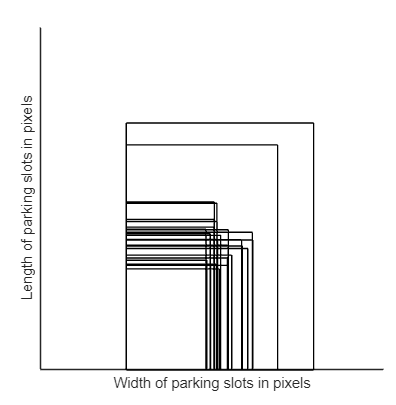
\includegraphics[]{figures/bboxPlot.png}
  \captionof{figure}{Plotted Bounding Boxes With Vertical Orientation}
  \label{fig:plottedRotatedBox}
\end{minipage}

The average of these box widths and lengths are calculated to be used to post-process the predicted bounding boxes to improve the predictions.

\begin{lstlisting}[]
averageLength = mean(adjustedClassifiedMean(:,4));
averageWidth = mean(adjustedClassifiedMean(:,3));
disp(averageLength)
disp(averageWidth)
\end{lstlisting}

The resulting average length is calculated as 79.8080 pixels and an average width of 60.3352 pixels. The screenshot of the output is in appendix C. These lengths will be used to adjust the predicted bounding box sizes in the next section. 

\subsubsection{Post-Process to Improve Predicting Bounding Box}

To improve predicted bounding boxes, a few assumptions was made. 

1. The width and length of each parking slot is constant, thus the average length and width calculated above will be used as the width and length of each parking space.

2. The car will take 80\% of the parking space, so the detections, or the predicted bounding box length, will be extended by 25\%.

The code used is based on the pseudocode provided.

\begin{lstlisting}[]

newBoxes = zeros(size(unrotatedClassifiedMeans));
aspectMore1=zeros(size(unrotatedClassifiedMeans));
aspectLess1=zeros(size(unrotatedClassifiedMeans));

% x,y, width, length
for i = 1:length(unrotatedClassifiedMeans)
    box = unrotatedClassifiedMeans(i, :);
    aspectRatio = box(3) / box(4);
    if aspectRatio > (averageLength/averageWidth) % for horizontally longer
        deltaX = (box(3) - (averageLength * 1.25));
        deltaY = (box(4) - averageWidth);
        newBoxes(i, 1) = box(1) + (deltaX / 2);
        newBoxes(i, 2) = box(2) + (deltaY / 2);
        newBoxes(i, 3) = averageLength*1.25;
        newBoxes(i, 4) = averageWidth;

        aspectMore1(i, 1) = box(1) + (deltaX / 2);
        aspectMore1(i, 2) = box(2) + (deltaY / 2);
        aspectMore1(i, 3) = averageLength*1.25 ;
        aspectMore1(i, 4) = averageWidth;
    else % for vertically longer boxes
        deltaX = (box(3) - averageWidth);
        deltaY = (box(4) - (averageLength * 1.25));
        newBoxes(i, 1) = box(1) + (deltaX / 2);
        newBoxes(i, 2) = box(2) + (deltaY / 2);
        newBoxes(i, 3) = averageWidth;
        newBoxes(i, 4) = averageLength*1.25;

        aspectLess1(i, 1) = box(1) + (deltaX / 2);
        aspectLess1(i, 2) = box(2) + (deltaY / 2);
        aspectLess1(i, 3) = averageWidth;
        aspectLess1(i, 4) = averageLength*1.25;
    end
end
\end{lstlisting}

The resulting new boxes were then plotted, with predicted boxes with an aspect ratio greater than average aspect ratio being colored green, aspect ratios being less than average aspect ratios colored cyan, and the ground truth bounding boxes being colored red. Figure \ref{fig:bboxplot1} shows this plot.

\newpage

\begin{minipage}{\linewidth}
  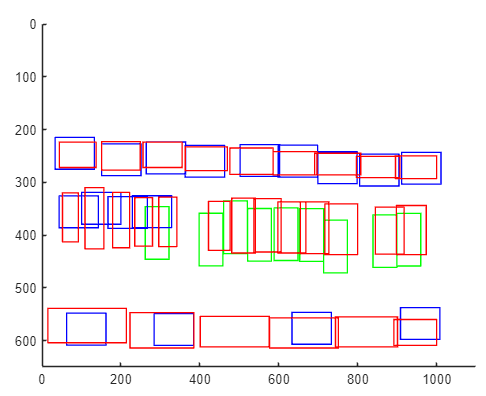
\includegraphics[height=\textheight/4,width=\textwidth/2]{figures/finalBbox1.png}
  \captionof{figure}{Predicted Bounding Boxes (blue and green) Plotted With Ground Truth (red)}
  \label{fig:bboxplot1}
\end{minipage}

A second plot was created without differing colors for different aspect ratios. Figure \ref{fig:bboxplot2} shows this plot.

\begin{minipage}{\linewidth}
  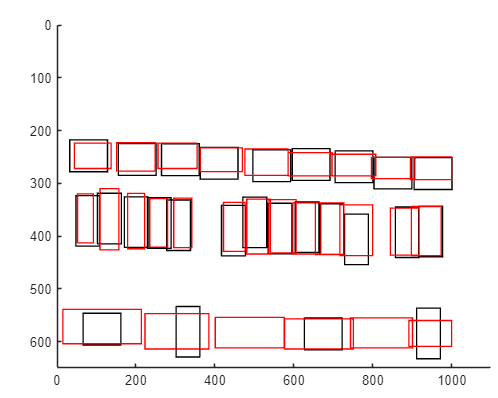
\includegraphics[height=\textheight/4,width=\textwidth/2]{figures/bboxplot2.png}
  \captionof{figure}{Predicted Bounding Boxes (black) Plotted With Ground Truth (red) Without Differentiation of Aspect Ratios}
  \label{fig:bboxplot2}
\end{minipage}

\begin{lstlisting}
figure;
xlim([0, 1100]);
ylim([0, 650]);
set(gca, 'YDir', 'reverse')
hold on;


for i = 1:size(newBoxes,1)
    rectangle('Position', aspectMore1(i,:), 'EdgeColor',
     'g', 'LineWidth', 1);
end

for i = 1:size(newBoxes,1)
    rectangle('Position', aspectLess1(i,:), 'EdgeColor',
     'blue', 'LineWidth', 1);
end

for i = 1:size(ParkingSlots,1)
    rectangle('Position', ParkingSlots(i,:), 'EdgeColor',
     'r', 'LineWidth', 1);
end
hold off;
\end{lstlisting}

The recall and precisions of the new post-processed boxes were then plotted in a similar way to the recall and precision plot of the initial predicted bounding boxes. Table \ref{fig:pProcessedPrecRec} shows the resulting precisions, recall, and average precisions of the post-processed predicted bounding boxes.

\newpage

\begin{minipage}{\linewidth}
  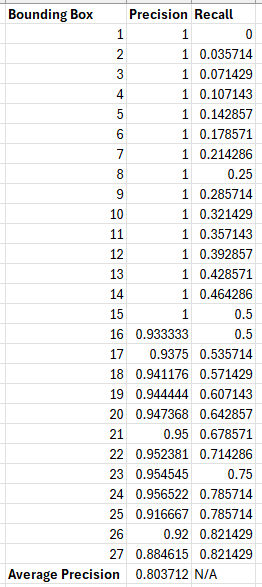
\includegraphics[]{figures/finalPrecRec.png}
  \captionof{figure}{Table of Precision, Average Precision, and Recall of Adjusted and Post-Processed Bounding Box Predictions}
  \label{fig:pProcessedPrecRec}
\end{minipage}

After the precisions and recalls were calculated, they are plotted using the following code.

\newpage

\begin{lstlisting}[]

newDetectionResults = detectionResults;
newDetectionResults.Boxes{1} = newBoxes;

[newAveragePrecision, newRecall, newPrecision] = evaluateDetectionPrecision
(newDetectionResults, groundTruthData);

figure;
plot(newRecall, newPrecision,'-x');
xlabel('Recall');
ylabel('Precision');
title(['Average Precision = ' num2str(newAveragePrecision) ]);
grid on;

\end{lstlisting}

The resulting plot is shown in figure \ref{fig:finalPlot}.

\newpage

\begin{minipage}{\linewidth}
  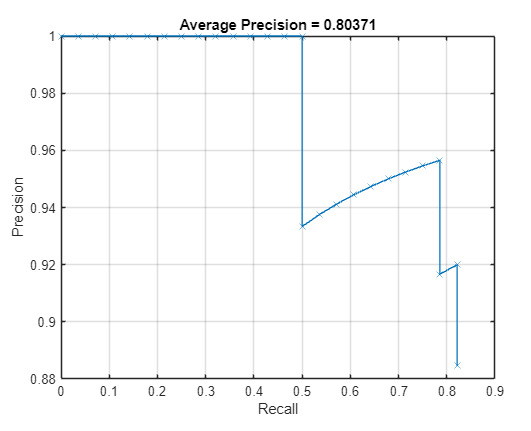
\includegraphics[height=\textheight/2,width=\textwidth/1]{figures/finalPrecRecPlot.png}
  \captionof{figure}{Plotted Recall vs Precision for Post-Processed Bounding Boxes}
  \label{fig:finalPlot}
\end{minipage}

\newpage

\section{Discussion}

\subsection{Accuracy, Precision, and Recall Evaluation}

\subsubsection{Car Detection With Resnet50 CNN Model}

The accuracy of the car detector model with the Resnet50 CNN model is highly accurate, as shown in figure \ref{fig:modelTraining}, showing that the model has high accuracy and low loss on both the training and development dataset. Furthermore, it is also shown to be able to generalize well to unseen datasets, as seen in the high accuracy in figure \ref{fig:confMatrix}.

\subsubsection{Parking Spot Delineation With FasterRCNN Model}

As seen in figure \ref{fig:modelIterations}, the accuracy in the training was quite high, with RPN and the overall model obtaining near perfect accuracy over a few thousand iterations. However, as shown in figure \ref{fig:bStreetPredictions}, it is not able to generalize very well towards unseen datasets, where it was only able to detect 17 of the 28 annotated parking spaces. Adding on more data by providing various other CCTV images of Barry Street did enhance the accuracy (see figure \ref{fig:clusterBox}), where the model was able to detect 26 of the 28 spaces.

While detection accuracy after providing the model with more data is better, the quality of the bounding boxes are not very accurate to the ground truth (see figure \ref{fig:unimprovedBoxes}). The resulting average precision was approximately 37\%, meaning that of all the instances the model predicted as a parking spot, about 37\% had correct bounding box predictions. The recall also tend to range from 3.5\% to 57\%, which means that about 3.5\% to 57\% of the specific bounding box were successfully detected as parking spots, while missing the remaining percentages for that specific bounding box. As the recall increases, the general trend is that there is an increase in precision as well, with only some points having decreased precision.

To improve the precision and recall of each bounding boxes, the improvements were made. The results will be discussed in the following section.

\subsection{Improvement Based on Assumptions}
The average precision decreased by about 43\%, which shows that the post-processed bounding boxes more accurately fit the annotated ground truth. The general trend of recall vs precision is also present in the post-processed plot (see figure \ref{fig:finalPlot}). 

To further investigate how the predicted boxes compare to the ground truth, figures \ref{fig:bboxplot1} and \ref{fig:bboxplot2} was created. In contrast to figure \ref{fig:unimprovedBoxes}, the post-processed boxes more closely resemble the ground truths. However, seeing figure \ref{fig:bboxplot1} shows that not all the parking spot orientations were identified. For example, two of the blue boxes on the bottom are vertically oriented, but the ground truth was that it should be a horizontal parking spot. This results in these predicted boxes having increased deviation from the ground truth. The bottom left parking spot was also much smaller than the others in the same row, which could be attributed to the image being cut off at that point, as seen in figure \ref{fig:bStreetPredictions}. 

For the vertically oriented predicted boxes, it correctly predicted all the the vertical parking spaces, although it did misclassify two horizontal boxes as vertical as mentioned above. However, for some of the boxes, there is a slight offset in the x and y coordinates, which causes increased errors.

Overall, the improvement through post-processing increaases the quality of predictions, through correctly identifiying orientations and adjusting the predicted bounding box sizes to be more accurate. However, there are still some problems with the assumptions. For example, the bottom row of Barry Street has a much larger parking spot thatn other areas, which does cause increased errors when only depending on average length and width. Furthermore, the intial predictions are also influential in identifying the correct aspect ratio of each bounding box (e.g., if the predicted width and length had an incorrect aspect ratio, the preprocessed boxes would also have incorrect aspect ratios). Nevertheless, using the assumptions and post-processing based on these assumptions does increase the average precision of the predictions.

\subsection{Challenges and Shortcomings}

One challenge in this report is correctly identifying aspect ratios. As stated above, due to the way the predictions were used in post-processing, the aspect ratios for some bounding boxes were not correctly identified. Generalizability is a core aspect in model training, and if a model was overfitted on certain datasets, they might not generalize well to unseen images. As such, although the assumptions and post-processing did help to improve some evaluation metrics, further post-processing could run the risk of overfitting. For example, if each bounding box was slowly shifted into its correct space and orientation by checking it against its corresponding ground truth box. This would greatly improve the metrics, but would also be an issue of overfitting.

Another challenge is interpreting the provided pseudocode as it was quite difficult to visualize the change. However, once it was understood that it was meant to account for horizontal and vertical orientations of parking, the resulting transformations were easier to visualize. 

\subsection{Scopes of Improvement}

To improve the report, the trained model could include training on the parking space orientations as an output. By directly training the output class of orientation itself, this could improve accuracy in post-processing. This would be in contrast to what this report has done, which is to calculate the aspect ratios based on predicted bounding boxes, which could cause errors to propagate. For instance, as described above, vertically oriented ground truth boxes are sometimes identified as horizontally oriented, which is an example of the error propagation (e.g., because the bounding box was more horizontal, the post-processing step also assumes it is horizontal regardless of the ground truth).

Another improvement could be to have more sophisticated assumptions. The provided assumptions are quite general, but as discussed above, does not apply to all parking spaces. Certain additional assumptions such as middle is always vertically oriented or the bottom row is always wider could further improve the evaluation metrics. However, this may not always be desired as it could cause overfitting. Nevertheless, if the goal was to obtain accurate predictions for one image to be used for some other purpose, this could be beneficial.

One final improvement is that there could be more sophisticated models, in which post-processed models could be fed back into the model to increase the generalizability of the model. However, designing such a model is outside the scope of this report and is a large project to undertake by itself.

\newpage

\section{Conclusions and Future Directions}

In conclusion, I have successfully investigated how neural networks and machine learning are applied in the field of computer vision. I have used pre-trained Restnet50 CNN and FasterRCNN models to perform car detection and delineation respectively. Furthermore, the performance of these models have been evaluated and visualized. After training, the FasterRCNN model was further fine-tuned in two ways. First was by providing it more data and averaging the predicted bounding boxes. The second was post-processing by using certain assumptions based on averaging length and width of all the bounding boxes. The results of post-processing was that the average precision decreased by about 43\%, and visual inspection of the plotted bounding boxes as seen in figure \ref{fig:bboxplot1} and \ref{fig:bboxplot2} shows that there was an improvement in the predicted bounding box areas to be closer to the ground truth. However, there are still issues in the predictions of bounding boxes due to two main points, that the assumption does not hold for all parking spaces and that errors are propagated from initial predictions due to the calculations of aspect ratios.

Future work can build on this report by implementing some of the suggestions in the scope of improvement section. While some of these are difficult and would require a large amount of work, such as the creation of a more sophisitcated model, some others can greatly improve the evaluation metrics, either by increasing assumptions or attempting to overfit the predictions based on the ground truth. However, these should be carefully considered on whether or not the risk of overfitting is suitable for the purposes of the desired study aim.

Nevertheless, this report has implemented all the steps provided in the specification and has achieved the aim of improving predictions provided by the provided models using various procedures. 

\newpage

\printbibliography

\newpage
\section{Appendix}

\noindent Appendix A - Table of the averaged bounding box means along with the average width and length.

\begin{minipage}{\linewidth}
  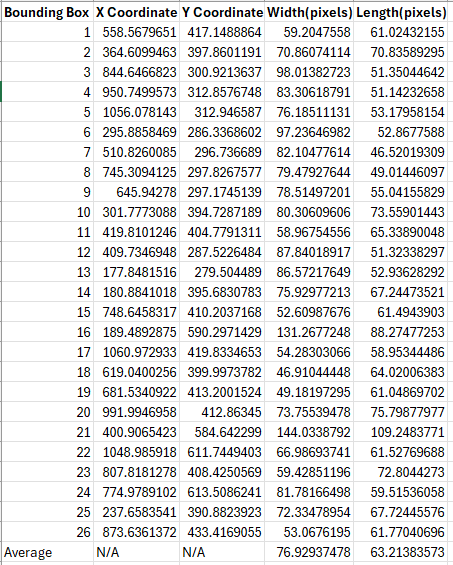
\includegraphics[]{figures/originalMeans.png}
  \captionof{figure}{Original Unadjusted Bounding Box Means}
  \label{fig:originalMeans}
\end{minipage}

\newpage

\noindent Appendix B - Table of adjusted bounding box means along with the average width and length

\begin{minipage}{\linewidth}
  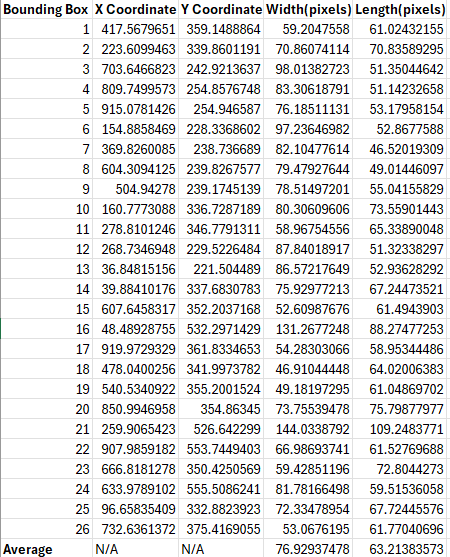
\includegraphics[]{figures/adjustedBoxes.png}
  \captionof{figure}{Adjusted Bounding Box Means}
  \label{fig:adjustedMeans}
\end{minipage}

\newpage

\noindent Appendix C - Screenshot of the average width and length of rotated and adjusted predicted bounding boxes

\begin{minipage}{\linewidth}
  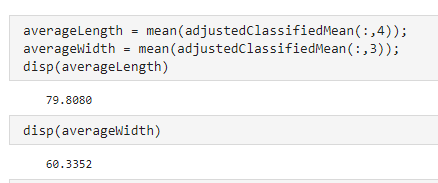
\includegraphics[]{figures/ssAverage.png}
  \captionof{figure}{Adjusted Predicted Bounding Boxes Width and Length}
  \label{fig:averageLW}
\end{minipage}

\newpage

\noindent Appendix D - Complete Code Used For Tasks 4 and 5 of the Assignment
\begin{lstlisting}[]

  % Task 4

  % x(1), y(2), length(3), width(4)
  disp(classifiedMean)
  adjustedClassifiedMean=classifiedMean
  adjustedClassifiedMean(:,1)=adjustedClassifiedMean(:,1)-141
  adjustedClassifiedMean(:,2)=adjustedClassifiedMean(:,2)-58
  
  detectionResults = table('Size',[1,2], ...
      'VariableTypes',{'cell','cell'}, ...
      'VariableNames', {'Boxes','Scores'})
  detectionResults.Boxes{1} = adjustedClassifiedMean;
  detectionResults.Scores{1} = classifiedScoreMean;
  disp(detectionResults)
  load("FinalCode\GroundTruthBarryStreet.mat")
  groundTruthData = table('Size',[1,1], ...
      'VariableTypes',{'cell'}, ...
      'VariableNames', {'Boxes'})
  groundTruthData.Boxes{1} = ParkingSlots
  [averagePrecision, recall, precision] = 
  evaluateDetectionPrecision(detectionResults, groundTruthData)
  figure;
  plot(recall, precision,'-x');
  xlabel('Recall');
  ylabel('Precision');
  title(['Average Precision = ' num2str(averagePrecision) ]);
  grid on;
  figure;
  xlim([0, 1100]);
  ylim([0, 650]);
  set(gca, 'YDir', 'reverse')
  hold on;
  
  for i = 1:size(adjustedClassifiedMean,1)
      rectangle('Position', adjustedClassifiedMean(i,:), 
      'EdgeColor', 'black', 'LineWidth', 1);
  end
  
  for i = 1:size(ParkingSlots,1)
      rectangle('Position', ParkingSlots(i,:), 'EdgeColor', 
      'r', 'LineWidth', 1);
  end
  hold off;
  
  
  %Task 5
  
  figure;
  hold on;
  axis equal;
  xlim([0, 200]);
  ylim([0, 200]);
  xlabel('Width of parking slots in pixels');
  ylabel('Length of parking slots in pixels');
  set(gca, 'XTick', [], 'YTick', []);
  
  %create a copy of adjustedClassifiedMeans before rotation for next task
  unrotatedClassifiedMeans=adjustedClassifiedMean
  
  for i = 1:size(adjustedClassifiedMean, 1)
      box =adjustedClassifiedMean(i, :);
      aspectRatio = adjustedClassifiedMean(i,4) 
      /adjustedClassifiedMean(i,3);
      if aspectRatio<1
          temp = adjustedClassifiedMean(i,3);
          adjustedClassifiedMean(i,3) =adjustedClassifiedMean(i,4);
          adjustedClassifiedMean(i,4) = temp;
          
          temp2=adjustedClassifiedMean(i,1);
          adjustedClassifiedMean(i,1)=adjustedClassifiedMean(i,2);
          adjustedClassifiedMean(i,2)=temp2;
          rectangle('Position', [50, 0, adjustedClassifiedMean(i,3),
          adjustedClassifiedMean(i,4)], 'EdgeColor', 'black');
      else
          rectangle('Position', [50, 0, adjustedClassifiedMean(i,3),
          adjustedClassifiedMean(i,4)], 'EdgeColor', 'black');
      end
        
  end
  
  hold off;
  averageLength = mean(adjustedClassifiedMean(:,4));
  averageWidth = mean(adjustedClassifiedMean(:,3));
  disp(averageLength)
  disp(averageWidth)
  
  newBoxes = zeros(size(unrotatedClassifiedMeans));
  aspectMore1=zeros(size(unrotatedClassifiedMeans));
  aspectLess1=zeros(size(unrotatedClassifiedMeans));
  
  % x,y, width, length
  for i = 1:length(unrotatedClassifiedMeans)
      box = unrotatedClassifiedMeans(i, :);
      aspectRatio = box(3) / box(4);
      if aspectRatio > (averageLength/averageWidth) % for vertically longer
          deltaX = (box(3) - (averageLength * 1.25));
          deltaY = (box(4) - averageWidth);
          newBoxes(i, 1) = box(1) + (deltaX / 2);
          newBoxes(i, 2) = box(2) + (deltaY / 2);
          newBoxes(i, 3) = averageLength*1.25;
          newBoxes(i, 4) = averageWidth;
  
          aspectMore1(i, 1) = box(1) + (deltaX / 2);
          aspectMore1(i, 2) = box(2) + (deltaY / 2);
          aspectMore1(i, 3) = averageLength*1.25 ;
          aspectMore1(i, 4) = averageWidth;
      else % for horizontally longer boxes
          deltaX = (box(3) - averageWidth);
          deltaY = (box(4) - (averageLength * 1.25));
          newBoxes(i, 1) = box(1) + (deltaX / 2);
          newBoxes(i, 2) = box(2) + (deltaY / 2);
          newBoxes(i, 3) = averageWidth;
          newBoxes(i, 4) = averageLength*1.25;
  
          aspectLess1(i, 1) = box(1) + (deltaX / 2);
          aspectLess1(i, 2) = box(2) + (deltaY / 2);
          aspectLess1(i, 3) = averageWidth;
          aspectLess1(i, 4) = averageLength*1.25;
      end
  end
  
  figure;
  xlim([0, 1100]);
  ylim([0, 650]);
  set(gca, 'YDir', 'reverse')
  hold on;
  
  
  for i = 1:size(newBoxes,1)
      rectangle('Position', aspectMore1(i,:), 'EdgeColor',
       'g', 'LineWidth', 1);
  end
  
  for i = 1:size(newBoxes,1)
      rectangle('Position', aspectLess1(i,:), 'EdgeColor',
       'blue', 'LineWidth', 1);
  end
  
  for i = 1:size(ParkingSlots,1)
      rectangle('Position', ParkingSlots(i,:), 'EdgeColor', 
      'r', 'LineWidth', 1);
  end
  hold off;
  
  figure;
  xlim([0, 1100]);
  ylim([0, 650]);
  set(gca, 'YDir', 'reverse')
  hold on;
  
  
  for i = 1:size(newBoxes,1)
      rectangle('Position', newBoxes(i,:), 'EdgeColor',
       'black', 'LineWidth', 1);
  end
  
  for i = 1:size(ParkingSlots,1)
      rectangle('Position', ParkingSlots(i,:), 'EdgeColor', 
      'r', 'LineWidth', 1);
  end
  hold off;
  
  
  newDetectionResults = detectionResults;
  newDetectionResults.Boxes{1} = newBoxes;
  
  [newAveragePrecision, newRecall, newPrecision] =
   evaluateDetectionPrecision(newDetectionResults, groundTruthData);
  
  figure;
  plot(newRecall, newPrecision,'-x');
  xlabel('Recall');
  ylabel('Precision');
  title(['Average Precision = ' num2str(newAveragePrecision) ]);
  grid on;

\end{lstlisting}

\end{document}